\section{Grafica}

Si representamos los datos obtenidos de la ejecución del programa
vemos como la gráfica representa una superficie con varios
niveles. Dichos niveles corresponden con las reglas que hemos definido
para el sistema, basándonos en las definidas en \cite{kosko1992}.

\begin{figure}
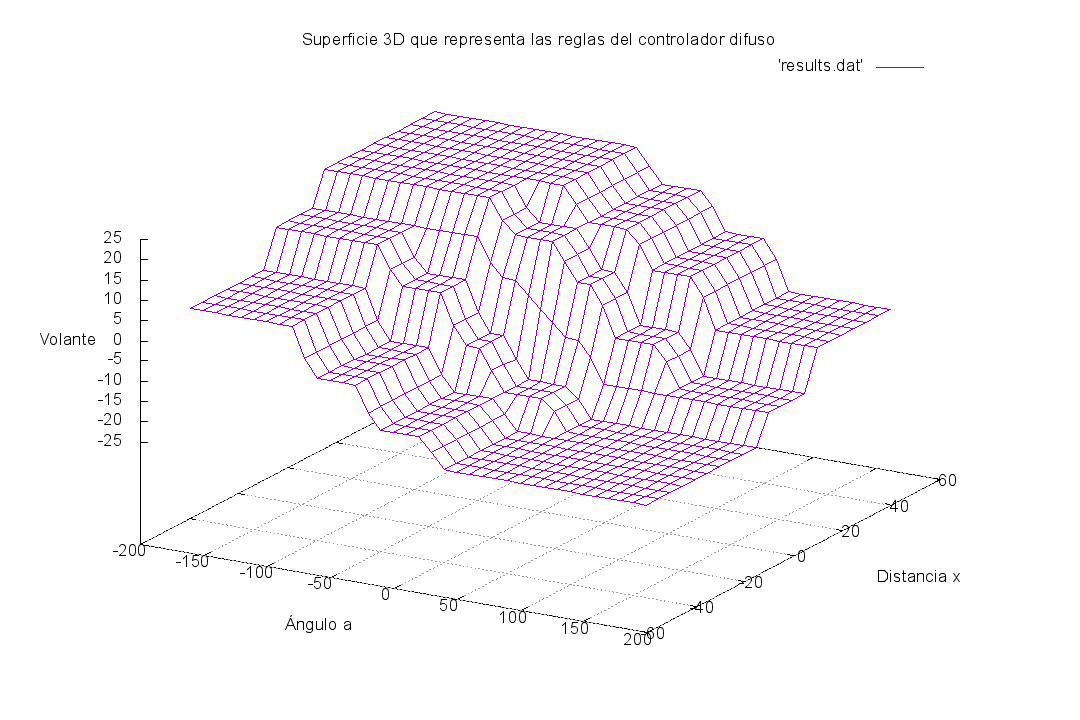
\includegraphics[width=\textwidth,height=\textheight,keepaspectratio]{superficie-resultado.png}
\caption{Representación gráfica de la salida del sistema para todos
  los valores posibles.}
\label{img:grafica2}
\end{figure}
